\section{Description of the Model}
 
\subsection{Environment}
\begin{wrapfigure}[18]{r}{0.5\textwidth}
  \centering
    \vspace{-0.4cm}
  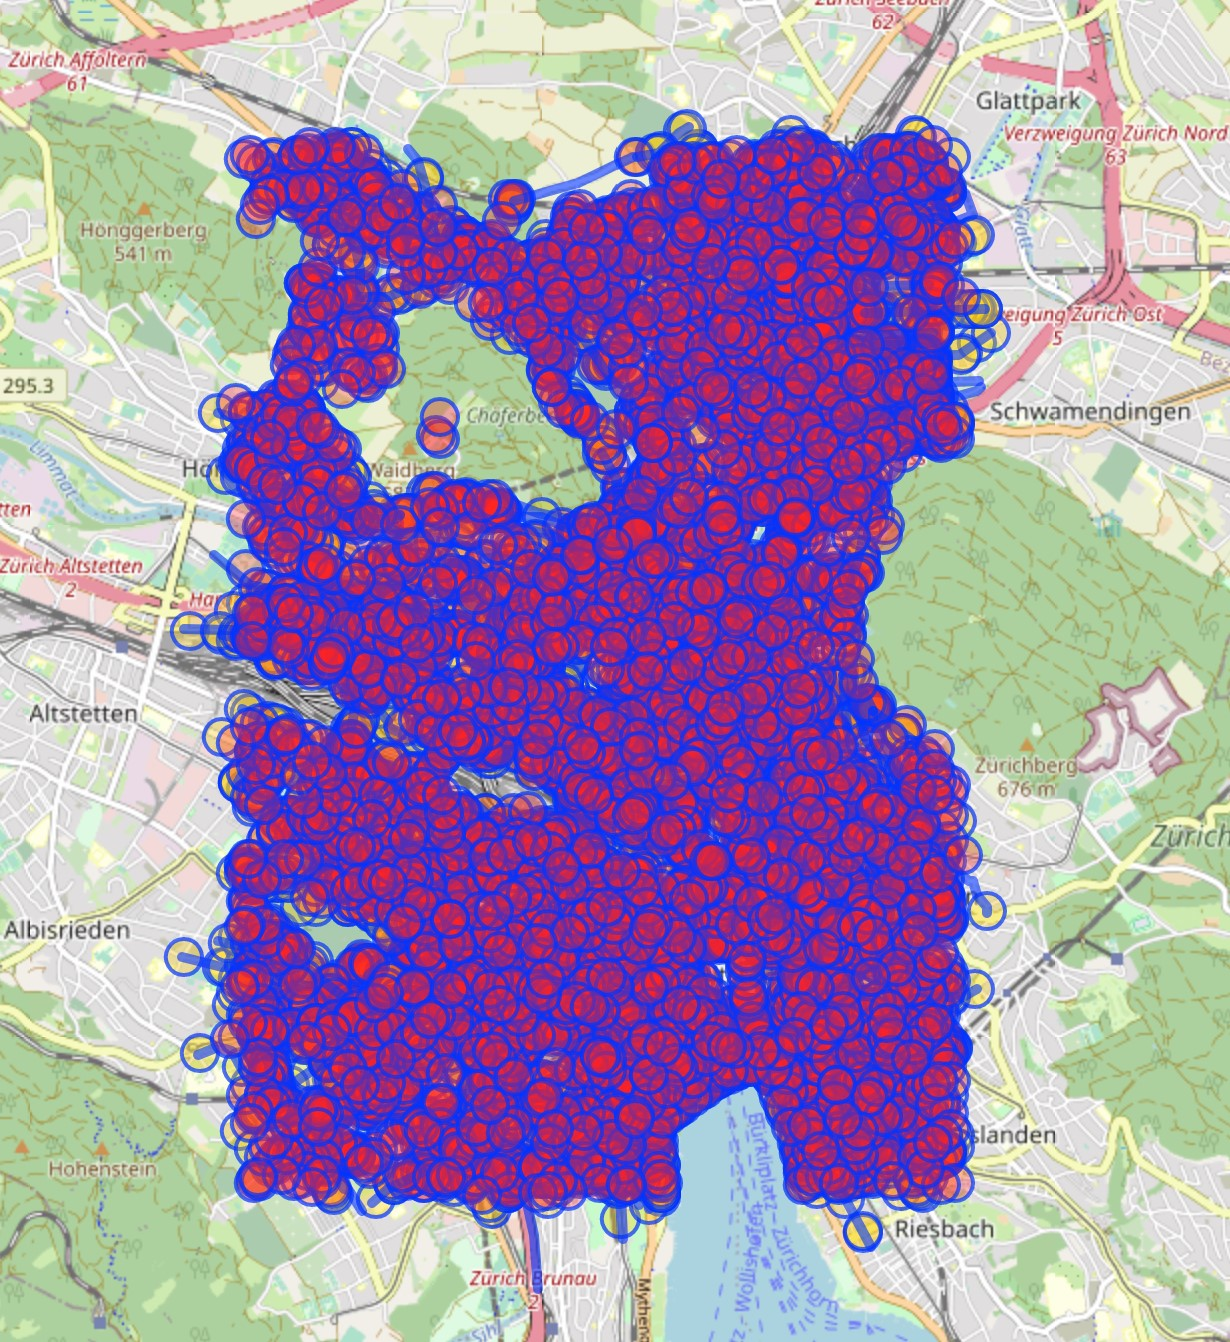
\includegraphics[width=\linewidth]{./figures/road-network.jpg}
  \captionsource{Modelled Road Network}{Screenshot taken from result of using our query in Overpass Turbo}\label{network}
\end{wrapfigure}

To understand the impact of bicycles on the traffic flow of cars we decided to make use of an Agent Based Model.  The realtime decisions made every day by thousands of travelers translate well into decisions to be made by Agents. Furthermore, traffic, and in particular car traffic, is constrained to roads, which makes for a very well defined environment. Our model environment is based on the road network of Zurich. Specifically, this model is constrained to the inner city of Zurich, using approximately a square of 4.5 by 8.9 kilometers of road network (see Fig.: \ref{network}).\\
The road network used contains streets ranging from larger highways and main roads such as the ``Limmatstrasse" but also smaller, more private roads.\\
In the model itself, the road network is split into streets and the intersections they are connected to. Both streets and intersections possess unique attributes. 

\subsubsection{Intersection}
The intersections are modeled as nodes in a graph with certain attributes. These attributes consist of an ID, a longitude and latitude attribute to denote its position, as well as which roads are incoming and outgoing. All intersections are modelled to be controlled through traffic lights. These are solely time controlled.

\subsubsection{Streets}
Each street is modeled as a directed edge between two intersections/vertices. Next to its ID, each street is uniquely determined by its start and end points, as well as its type. The type refers to the vehicle type which can use the road, which is ``bike", ``car" or ``mixed". Therefore there is at most one edge available for each agent type between two pairs of vertices.\\
A street has several attributes. One is the number of lanes, which is assumed to be one as default, in case there is no further information in the raw data. The other attributes are the speed limit, which is assumed to be 50 km/h as a default, as well as the length of the road, which is calculated using the coordinates of its endpoints.

\subsection{Agents}\label{agentDesc}
\subsubsection{General Attributes}
The agents consist of two types, cyclists and cars. Each agent has a start and end intersection, which determines the start and end point of its journey. Furthermore, an agent has several attributes determining the behavior. The attributes have an interval for cyclists and for cars, which it is uniformly chosen out of (see Tab.: \ref{tab:agentAttr.}). Each agent possesses an additional attribute, that tells it at what time to start its journey. This value is given in seconds. 

\begin{table}[H]
\begin{center}
\begin{tabularx}{\linewidth}{C|C|C|C|C|C}
    & \textbf{Length} ($m$) & \textbf{Maximum Velocity} ($km/h$) & \textbf{Accel-} \textbf{eration} ($m/s^2$) & \textbf{Decel-} \textbf{eration} ($-m/s^2$) & \textbf{Acceleration Exponent}\\
    \hline
    \textbf{Cars} & $[3.5, 5]$ & $[100, 250]$ & $[1.5, 5]$ & $[2, 6]$ & $[8, 12]$\\
    \hline
    \textbf{Bicycles} & $[1.5, 2.5]$ & $[10, 35]$ & $[0.5, 1.5]$ & $[1, 3]$ & $[8, 12]$
\end{tabularx}
\caption{Possible Ranges for Agent Attributes}\label{tab:agentAttr.}
\end{center}
\end{table}
\vspace{-0.75cm}
The agents are generated hourly and for each agent in this hour, the exact time of departure is uniformly chosen. The absolute amount of agents per hour is calculated relative to the area of the map. We assume that for every 4'000$m^2$ of the map, one agent spawns per hour. This number was chosen, since in 2022 there where 182'805  motorized vehicles registered in the city of Zurich. \cite{carAmount} About 57\% of daily kilometers is absolved through motorized individual transport. \cite{verhalten} Therefore, we made the assumption, that every second vehicle is moved once a day, resulting in around 90'000 agents spawned over the course of the simulation. Most of them travel in the span of around 12 hours, which we made the length of the simulation. This leaves us with one agent spawned per hour and 4'000$m^2$, to achieve a total of approximately 90'000 agents over twelve hours on the used map.
\subsubsection{Agent Behaviour}
Every agent wishes to travel from its start to end point as quickly as possible. At the beginning of the simulation, the shortest paths between all nodes are calculated. The agent chooses this path for their journey and uses the appropriate streets to travel from intersection to intersection. On the street, the agent accelerates or decelerates to maintain a safe distance from the next agent. If the street has multiple lanes, the agent will choose the lane with the most space available. Bikes are required to stay in the right lane on large streets unless the street is marked as bike-only. Furthermore, agents can overtake other agents (i.e. a car overtakes a slower bike), provided there is a high enough difference in speed and there is a free lane on the overtaking agent's left. The equation to describe the motion of the agents is the following: \cite{helbl}
\begin{align*}
\dot{x}_\alpha &= v_\alpha\\
\dot{v}_\alpha &= a\left[ 1 - \left( \frac{v_\alpha}{v_0}\right)^\delta - \left(\frac{s^*(v_\alpha, \Delta v_\alpha)}{s_\alpha} \right)^2 \right]
\end{align*}

Where $s^*(v, \Delta v)$ is the dynamic desired distance defined by:
\begin{equation*}
s^*(v, \Delta v) = s_0 + v T +  \frac{v\Delta v}{2\sqrt{a\cdot b}}
\end{equation*}

The above-used variables have the following meanings, where $\alpha$ denotes our agent:
\begin{align*}
x_\alpha &= \text{ distance from agent to next intersection}\\
v_\alpha &= \text{ velocity to be achieved by agent}\\
v_0 &= \text{ current speed}\\
\Delta v_\alpha &= \text{ difference in velocity either to next agent or to intersection}\\
a &= \text{ acceleration of agent}\\
b &= \text{ deceleration of agent}\\
\delta &= \text{ acceleration coefficient}\\
s_\alpha &= \text{ current distance to next object}\\
s_0 &= \text{ minimum distance to next object}\\
T &= \text{ time}
\end{align*}

